%███████████████████████████████████████████████████████████████████
\appendix
\chapter{}

%███████████████████████████████████████████████████████████████████
%███████████████████████████████████████████████████████████████████
\section{Four-Vectors}\label{sect: Four-Vectors}

Four-vectors are vectors with 4 components, with 3 of them linked to the spacial dimensions and 1 linked to the time dimension.
The simplest example is the four-position which is defined as

\begin{equation}
	\mathbf{X}_4 = \begin{pmatrix}
		ct \\
		x  \\
		y  \\
		z
	\end{pmatrix}
\end{equation}

The first quantity being the time component multiplied by the speed of light, giving the same units as the other components.
The other three components being the spacial coordinates.

These use another quantity called the Minkowski metric, that when the applied to the four vector gives an invariant quantity

The Minkowski metric is given as

\begin{equation}
	g_{\mu\nu} = \begin{pmatrix}
		-1 & 0 & 0 & 0 \\
		0  & 1 & 0 & 0 \\
		0  & 0 & 1 & 0 \\
		0  & 0 & 0 & 1
	\end{pmatrix}
\end{equation}

by design all four vectors

The reason they are use is becuase they make the calculations easier in some use cases, and the

a quantity used in special relativity, that can make it easier to work with invariant under Lorentz transformations, ensuring that the laws hold true in all inertial reference frames.

\begin{equation}
	g_{\mu\nu} = \begin{pmatrix}
		-1 & 0 & 0 & 0 \\
		0  & 1 & 0 & 0 \\
		0  & 0 & 1 & 0 \\
		0  & 0 & 0 & 1
	\end{pmatrix}
\end{equation}

Euclidean space uses the metric tensor

\begin{equation}
	g_{\mu\nu} = \begin{pmatrix}
		1 & 0 & 0 & 0 \\
		0 & 1 & 0 & 0 \\
		0 & 0 & 1 & 0 \\
		0 & 0 & 0 & 1
	\end{pmatrix}
\end{equation}


%███████████████████████████████████████████████████████████████████
%███████████████████████████████████████████████████████████████████
\section{Cheat Sheets}\label{sect: Cheat Sheets}

*** here I will give cheat sheets, and steps to carry out what I have gone through previously

%███████████████████████████████████████████████████████████████████
%███████████████████████████████████████████████████████████████████
\section{Extras}\label{sect: Extras}

***

\begin{equation}
	\left( \frac{\partial^2}{\partial x^2} + \frac{\partial^2}{\partial y^2} + \frac{1}{\gamma^2} \frac{\partial^2}{\partial z^2} \right) \frac{1}{L} = 0
\end{equation}

is this an invariant quantity?

***

%███████████████████████████████████████████████████████████████████
%███████████████████████████████████████████████████████████████████
%███████████████████████████████████████████████████████████████████
\chapter{Ways to get inverse square laws}\label{ch: Ways to get inverse square laws}

*** The quantities we will derive in this chapter are not wrong in themselves, but could be used to wrongly state that they are the cause of any physical phenomenon beyond what they mathematically describe.
*** The quantities we will derive in this chapter are not meant derived due to the thought they might have physical consequences.

*** You will notice that I for some reason am keen to find quantities that have an inverse square law (quantities that are inversely proportional to the distance from a source) in a sources rest frame, and then extending it to the case of a moving source.

*** the reason for this because i know the electrodynamic field uses photons as the force carriers from a source, and for the case of a stationary charge in classical electrodynamics, the force a stationary charge applies to another is inversely proportional to the square of the distance between them.

*** my expectation is not to find discover something profound by looking at other quantities with this inverse square law

*** but to just see how many reasonable ways I can get it, because I found it an interesting challenge

*** and if there was something to get out of it that would be an added extra, a but a very long shot

*** but they are more done for the sake of curiousity, and to invoke ones imagination/creativity

*** some of these may have a bit of reasoning and some may seem to be a bit of a stretch to get to, and few jumps in logic missing.

This chapter will look at a source that continuously emits evenly distributed pulses of light radially outwards, giving a source at rest a "field" of light that spreads out evenly the further it is from the source.
The amount this light is spread out on the sphere that the light pulse creates, at a distance $r$, is proportional to the inverse square of the distance, $1/r^2$.
This inverse square law is used to describe how the classical forces between two masses or charges dissipate with the distance between them.
But, this scalar density is not the only way to get an inverse square law.
In this chapter we will look at other properties of a field of continuously emitted light, and we will see that they can also give you an inverse square law.
The other ways in which we will find this inverse square law include deconstructing the light's density into a vector of the density in each of the unit vectors of the spherical polar coordinate's directions and applying the Jacobian matrix, and also separately by using the gradient operator, this will give two different ways in which to measure of the rate of change of the density in all directions.
We will also get the inverse square law by using the Jacobian matrix on the velocity vector of light at each point in the light field, which will give us a measure of the rate of change of the velocity of light in all directions.
For each of these we will also find the corresponding quantities for the case of a moving source, with the help of the previous chapter.

%███████████████████████████████████████████████████████████████████
\section{Light Density Deconstructed into Vector}\label{sect: Field Vector Density}

Here we will try something a little different to see if there is anything interesting to get out of it. The quantity that we are about to describe, is not something that is used in physics.

Instead of the volume density we previously had, we could describe the density of light in three perpendicular directions, with a density in the direction of the light's propagation $D_c$ given in equation \eqref{eq: denisty of light parallel to propagation}, and by deconstructing the surface element's density $D_\sigma$, from equation \eqref{eq: denisty of light in surface element} equally ($\sqrt{D_\sigma}$) into the two directions $\hat{\alpha}$ and $\hat{\phi}$, which are perpendicular to the direction of light's propagation $\hat{c}$.

The radial density is constant, and for the density in each of the angular directions we will split the inverse square law equally between them, by taking the square root of it.

% instead of
% \begin{equation}
% 	\nabla = \frac{\partial}{\partial r} \underline{e}_r + \frac{1}{r} \frac{\partial}{\partial\theta} \underline{e}_\theta + \frac{1}{r \sin{\theta}} \frac{\partial}{\partial\phi} \underline{e}_\phi
% \end{equation}

\begin{equation}
	\label{eq: density vector}
	\mhl{
		\begin{aligned}
			\underline{D} & \color{gray} = D_{c} \hat{\underline{c}} + \sqrt{D_{\sigma}}  \hat{\underline{\alpha}} + \sqrt{D_{\sigma}} \hat{\underline{\varphi}}                                           \\
			              & = {\gamma}\left(1 + \dfrac{u}{c}\frac{\gamma z}{L}\right) k_c \hat{\underline{c}} + \frac{k_\sigma}{L} \hat{\underline{\alpha}} + \frac{k_\sigma}{L} \hat{\underline{\varphi}}
		\end{aligned}
	}
\end{equation}

*** note that $k_\sigma \rightarrow k_\sigma^2$

The components of this density vector are the densities of light in the corresponding unit vector directions

Now we will check two ways in which we can get an inverse square law from this density vector.

First, from calculating the norm of a Jacobian matrix of this density vector (a matrix of partial derivatives), it will be a measure of the rate of change of these vector density elements of light in all direction.
These density vector elements are in the directions parallel and perpendicular to the light's propagation, and we are looking at the rate of change of these with respect to x, y and z-directions.

The second way in which we will get the inverse square law, will be, by taking the magnitude of the density vector and then calculating its directional derivative $ \nabla  \| \underline{D} \| \cdot \hat{\underline{c}}$.
It is a measure of the rate of change of the magnitude of the light's density vector in the direction of the light's propagation.

%███████████████████████████████████████████████████████████████████
\section{Jacobian of Density Vector}\label{sect: Jacobian matrix of the Density vec}

*** look at 4-current $(c\rho, D_c, D_\alpha, D_\varphi)= (c\rho, \mathbf{J})$

*** where $\mathbf{J}=(D_c,\sqrt{D_\sigma},\sqrt{D_\sigma})$ is the current density of light in their corresponding directions, and $\rho$ is the volume density of light

*** actually $\mathbf{J}= \rho \mathbf{\hat{c}}$ where again $\rho$ is the volume density of light

*** or outer product with gradient

*** maybe use 4d jacobian

*** or use outer product with 4-gradient

*** with density's time component being a quantity that is a constant with respect to time

We will now check the Jacobian matrix of the density vector.
The Jacobian for our density vector is a matrix of partial derivatives of each of the density vector's components with respect to each coordinate, i.e. the rate of change of each component with respect to each coordinate, given as

\begin{equation}
	J = \begin{bmatrix}
		\frac{\partial D_{1}}{\partial x} & \frac{\partial D_{1}}{\partial y} & \frac{\partial D_{1}}{\partial z} \\
		\frac{\partial D_{2}}{\partial x} & \frac{\partial D_{2}}{\partial y} & \frac{\partial D_{2}}{\partial z} \\
		\frac{\partial D_{3}}{\partial x} & \frac{\partial D_{3}}{\partial y} & \frac{\partial D_{3}}{\partial z}
	\end{bmatrix}
\end{equation}

% \begin{equation}
% 	J = \begin{bmatrix}
% 		\frac{\partial D_{1}}{\partial r} & \frac{\partial D_{1}}{\partial \alpha_0} & \frac{\partial D_{1}}{\partial \varphi_0} \\
% 		\frac{\partial D_{2}}{\partial r} & \frac{\partial D_{2}}{\partial \alpha_0} & \frac{\partial D_{2}}{\partial \varphi_0} \\
% 		\frac{\partial D_{3}}{\partial r} & \frac{\partial D_{3}}{\partial \alpha_0} & \frac{\partial D_{3}}{\partial \varphi_0}
% 		\end{bmatrix}
% 		= \begin{bmatrix}
% 			0 & 0 & 0 \\
% 			- \frac{k_\theta}{r^2} & 0 & 0 \\
% 			- \frac{k_\phi}{r^2} & 0 & 0
% 			\end{bmatrix}
% \end{equation}

% or

% \begin{equation}
% 	J = - \frac{k_{\Omega}}{r^3}
% 	\begin{bmatrix}
% 		0 & 0 & 0 \\
% 		x & y & z \\

% 		x & y & z
% 	\end{bmatrix}
% \end{equation}


% We can then find the norm of the Jacobian matrix to be


% \begin{equation}
% 	\begin{aligned}
% 		\| J \| & \color{gray} =   \frac{k_\sigma}{r^3}\sqrt{2x^2+2y^2+2z^2} \\
% 		        & =  \frac{ \sqrt{2} k_\sigma}{r^2}
% 	\end{aligned}
% \end{equation}


% This is again found to be an inverse square law, with the proportionality constant being $\sqrt{2}k_\sigma$.
% It is a measure of the total rate of change of light's density in space.
% Now let us see this for a moving source

% %█████████████
% \subsubsection{For a Moving Source:}\label{subsubsect: General Equations for Moving Source 2}

% \begin{equation}
% 	\begin{aligned}
% 		\sqrt{\frac{D_{\sigma}}{L_p^2}} & \color{gray} =  {\gamma}\left(1 + \dfrac{u}{c}\frac{\gamma z}{L}\right) \cdot \frac{1}{\gamma \left( 1 + \frac{u}{c} \frac{\gamma z}{L} \right) L} \\
% 		                              & = \frac{1}{L}
% 	\end{aligned}
% \end{equation}


Using the density vector from equation \eqref{eq: density vector}, remembering that $ L=\sqrt{x^2+y^2+\gamma^2 z^2}$ and setting $\beta = - u/c$, we can find the Jacobian matrix of the density vector.

%█████████████████
\begin{derivation}

	%%% checked with
	% https://www.wolframalpha.com/input?i=gradient+of+%28+g+%281+-b+%28g+z%29%2F%28+sqrt%28x%5E2%2By%5E2%2B+g%5E2+z%5E2%29%29+%29+M%2C+J+%2F++sqrt%28x%5E2%2By%5E2%2B+g%5E2+z%5E2%29%2C+K+%2F++sqrt%28x%5E2%2By%5E2%2B+g%5E2+z%5E2%29+%29+
	%%% or
	% https://www.wolframalpha.com/input?i2d=true&i=Divide%5Bd%2Cdx%5D+g+%5C%2840%291+-b+*+%5C%2840%29Divide%5Bg*z%2CSqrt%5BPower%5Bx%2C2%5D%2BPower%5By%2C2%5D%2B+Power%5Bg%2C2%5D*Power%5Bz%2C2%5D%5D%5D%5C%2841%29%5C%2841%29
	% https://www.wolframalpha.com/input?i2d=true&i=Divide%5Bd%2Cdz%5D+g+%5C%2840%291+-b+*+%5C%2840%29Divide%5Bg*z%2CSqrt%5BPower%5Bx%2C2%5D%2BPower%5By%2C2%5D%2B+Power%5Bg%2C2%5D*Power%5Bz%2C2%5D%5D%5D%5C%2841%29%5C%2841%29

	\begin{equation}
		\begin{aligned}
			J & =
			\begin{bmatrix}
				\frac{\partial D_{1}}{\partial x} & \frac{\partial D_{1}}{\partial y} & \frac{\partial D_{1}}{\partial z} \\
				\frac{\partial D_{2}}{\partial x} & \frac{\partial D_{2}}{\partial y} & \frac{\partial D_{2}}{\partial z} \\
				\frac{\partial D_{3}}{\partial x} & \frac{\partial D_{3}}{\partial y} & \frac{\partial D_{3}}{\partial z}
			\end{bmatrix}
			\\
			  & =  \frac{1}{L^3}
			\begin{bmatrix}
				k_c \gamma^2 \beta xz & k_c \gamma^2 \beta yz & - k_c \gamma^2 \beta (x^2 +y^2) \\
				-k_\sigma x           & -k_\sigma y           & -k_\sigma\gamma^2 z             \\
				-k_\sigma x           & -k_\sigma y           & -k_\sigma\gamma^2 z
			\end{bmatrix}
		\end{aligned}
	\end{equation}

	then we have

	%checked
	\begin{equation}
		\begin{aligned}
			\| J \| & = \frac{1}{L^3} \sqrt{ 2 k_\sigma^2 L^2 + k_c^2 \gamma^4 \beta^2  (x^2+y^2)( x^2 + y^2 + z^2 )}          \\
			        & = \frac{1}{L^2} \sqrt{ 2 k_\sigma^2 + k_c^2 \gamma^4 \beta^2 (x^2+y^2) \frac{\|\underline{l}\|^2}{L^2} }
		\end{aligned}
	\end{equation}

\end{derivation}
%███████████████

if it happens to be that $k_c\approx 0$, then we would get

\begin{equation}
	\| J \| = \frac{ \sqrt{2} k_\sigma}{L^2}
\end{equation}

We can see this quantity for a rest and moving source in the figure below, it is the same as figure (\ref{fig: Density of light for surface element}).

%█████████████
\begin{figure}[H]
	\centering
	\begin{subfigure}{0.45\textwidth}
		\centering
		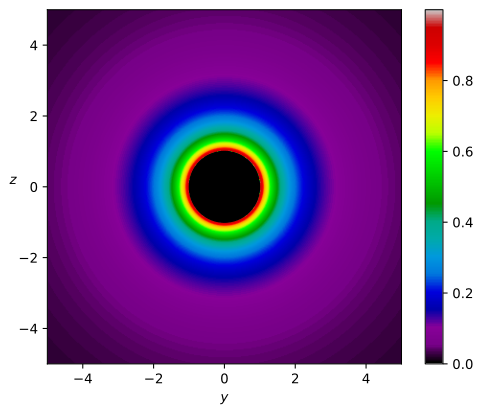
\includegraphics[width=\textwidth]{images/pdf/Density_of_Light_from_Rest_Source.pdf}
		\caption{Rest Source}
		\label{subfig_1: jacobian of vector density}
	\end{subfigure}
	\begin{subfigure}{0.45\textwidth}
		\centering
		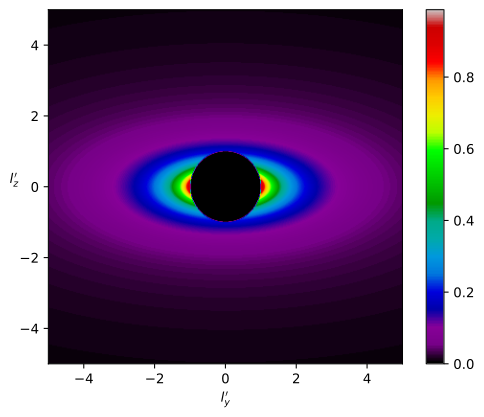
\includegraphics[width=\textwidth]{images/pdf/Rate_of_Change_of_Vector_Density_of_Light_from_Moving_Source.pdf}
		\caption{Moving Source}
		\label{subfig_2: jacobian of vector density}
	\end{subfigure}
	\caption{\textbf{Magnitude of light density's Jacobian}. This Figure shows a measure of the total rate of change of the vector density of the emitted light from a source in all directions, $\| \underline{J} \|$, plotted in the 2d y-z plane, the value of this goes to infinity as we get closer to the source, so for us to be able to color the graph nicely we needed to remove the center, shown by the black circle in the center.}
	\label{fig: jacobian of vector density}
\end{figure}
%███████████

%███████████████████████████████████████████████████████████████████
\section{Density Vector Magnitude's Directional Derivative}\label{sect: Norm of the Gradient of the Density Vector Magnitude}

We could also find the rate of change of the magnitude of the density vector in the direction of the light's propagation, given by the directional derivative, which is

\begin{equation}
	\nabla_c \| \underline{D} \| = \nabla \| \underline{D} \| \cdot \hat{\underline{c}}
\end{equation}

It is the gradient of $\|D\|$ in the direction $\hat{c}$.

% \begin{derivation}

% 	The magnitude of the density vector, is given by

% 	\begin{equation}
% 		\| \underline{D} \| = \sqrt{k_c^2 + \frac{2 k_\sigma^2}{r^2} }
% 	\end{equation}

% 	And the gradient of this is

% 	\begin{equation}
% 		\nabla \| \underline{D} \| =
% 		\begin{pmatrix}
% 			\frac{\partial}{\partial x}  \| \underline{D} \| \\
% 			\frac{\partial}{\partial y}  \| \underline{D} \| \\
% 			\frac{\partial}{\partial z}  \| \underline{D} \|
% 		\end{pmatrix}
% 		% =
% 		% \begin{pmatrix}
% 		% 	-\frac{2 k_\sigma^2 x}{r^4\sqrt{k_c^2 + \frac{2 k_\sigma^2}{r^2} }} \\
% 		% 	-\frac{2 k_\sigma^2 y}{r^4\sqrt{k_c^2 + \frac{2 k_\sigma^2}{r^2} }} \\
% 		% 	-\frac{2 k_\sigma^2 z}{r^4\sqrt{k_c^2 + \frac{2 k_\sigma^2}{r^2} }}
% 		% \end{pmatrix}
% 		= -\frac{2 k_\sigma^2}{r^3\sqrt{r^2k_c^2 + 2 k_\sigma^2 }}
% 		\begin{pmatrix}
% 			x \\
% 			y \\
% 			z
% 		\end{pmatrix}
% 	\end{equation}

% 	now taking the dot product with the direction of the light's propagation, which for the rest case is the unit vector of the position vector, with this we will get

% 	\begin{equation}
% 		\nabla_c \| \underline{D} \| = \nabla \| \underline{D} \| \cdot \hat{\underline{c}} = - \frac{2 k_\sigma^2}{r^2\sqrt{r^2 k_c^2 + k_\sigma^2}}
% 	\end{equation}

% \end{derivation}


% checking in cartesian Coordinates:
% \begin{equation}
% 	\underline{\hat{\text{${r}$}}} =
% 	\begin{pmatrix}
% 		\sin\theta \, \cos\phi \\
% 		\sin\theta \, \sin\phi \\
% 		\cos\theta            \\
% 	\end{pmatrix},
% 	\underline{\hat{\text{$\theta$}}} =
% 	\begin{pmatrix}
% 		\cos\theta \, \cos\phi \\
% 		\cos\theta \, \sin\phi \\
% 		-\sin\theta            \\
% 	\end{pmatrix},
% 	\underline{\hat{\text{$\phi$}}} =
% 	\begin{pmatrix}
% 		-\, \sin\phi             \\
% 		\hphantom{-} \, \cos\phi \\
% 		0                        \\
% 	\end{pmatrix}
% \end{equation}
% \begin{equation}
% 	\underline{\hat{\text{${D}$}}} = \frac{1}{r\rho}
% 	\begin{pmatrix}
% 		ax\rho +bxz - byr  \\
% 		ay\rho + byz + bxr \\
% 		az - b(x^2+y^2)
% 	\end{pmatrix}
% \end{equation}
% with $r=\sqrt{x^2+y^2+z^2}$ and $\rho=\sqrt{x^2+z^2}$

% %█████████████
% \subsubsection{General Equations for Moving Source}\label{subsubsect: General Equations for Moving Source 3}

Like we did for the previous section we will take $k_c \approx 0$, as the equations get very complex otherwise.
It is also required for us to get the inverse square law to hold for the rest source.

\begin{derivation}

	using $k_c \approx 0$ simplifies the density vector magnitude to

	\begin{equation}
		\| \underline{D} \| = \frac{k_\sigma}{L}
	\end{equation}

	giving the gradient of this as

	\begin{equation}
		\nabla \| \underline{D} \| = -\frac{k_\sigma}{L^3}
		\begin{pmatrix}
			x \\
			y \\
			\gamma^2 z
		\end{pmatrix}
	\end{equation}

	now taking the dot product with the direction of the light's propagation, in the case of a moving source we use the unit vector of equation \eqref{eq: light pulse velocity transform}, giving

	\begin{equation}
		\begin{aligned}
			\nabla \| \underline{D} \| \cdot \underline{\hat{c}}
			 & = -\frac{k_\sigma}{L^3}
			\begin{pmatrix}
				x \\
				y \\
				\gamma^2 z
			\end{pmatrix}
			\cdot
			\frac{1}{ \gamma \left( 1 + \frac{u}{c} \frac{\gamma {z}}{L} \right) }
			\begin{pmatrix}
				\frac{{x}}{L} \\
				\frac{{y}}{L} \\
				\gamma \left( \frac{\gamma {z}}{L} + \frac{u}{c} \right)
			\end{pmatrix}                                              \\
			 & = -\frac{2k_\sigma}{\gamma\left(1-\beta\frac{\gamma z}{L}\right)L^4} \left( x^2 + y^2 + \gamma^4 z^2 - \gamma^3 \beta z L \right)
		\end{aligned}
	\end{equation}

\end{derivation}




% %█████████████████
% \begin{derivation}

% 	\begin{equation}
% 		\|\underline{D}\| = \sqrt{ \frac{k_\sigma^2}{L^2} + k_c^2 \gamma^2\left( 1-\beta \gamma \frac{z}{L} \right)^2 }
% 	\end{equation}

% 	% https://www.wolframalpha.com/input?i=Grad%5Bsqrt%28+%28a%5E2%29%2F%28x%5E2%2By%5E2%2B+g%5E2+z%5E2%29+%2B+k%5E2+g%5E2+%28+1-b+g+%28z%29+%2F+sqrt%28x%5E2%2By%5E2%2B+g%5E2+z%5E2%29+%29%5E2+%29+%5D

% 	\begin{equation}
% 		\nabla \|\underline{D}\| = \frac{1}{L^3 \sqrt{\frac{k_\sigma^2}{L^2} + k_c^2\gamma^2(1-\gamma\beta\frac{z}{L})^2}}
% 		\begin{pmatrix}
% 			-\frac{x}{L} k_\sigma^2 + k_c^2 \gamma^3 \beta (1-\gamma\beta \frac{z}{L}) xz \\
% 			-\frac{y}{L} k_\sigma^2 + k_c^2 \gamma^3 \beta (1-\gamma\beta \frac{z}{L}) yz \\
% 			-\gamma^2\frac{z}{L} k_\sigma^2 - k_c^2 \gamma^3 \beta (1-\gamma\beta \frac{z}{L}) (x^2 + y^2)
% 		\end{pmatrix}
% 	\end{equation}

% 	$H=\beta \gamma^3 k_c^2 (1-\beta\frac{\gamma z}{L})$

% \end{derivation}
% %███████████████


% % \begin{equation}
% % 	\Big\| \nabla \|\underline{D}\| \Big\| = \frac{1}{L^2\sqrt{k_a^2+ \gamma^2(1-\beta\gamma\frac{z}{L})^2 L^2k_c^2}} \sqrt{ \frac{x^2+y^2+\gamma^4 z^2}{L^2} k_a^4 + \frac{x^2 + y^2}{L^2} \left( \frac{\|\underline{l}\|^2}{L^2} H^2 + 2 (\gamma^2-1)k_a^2 \frac{z}{L} H \right) }
% % \end{equation}

% If we take the norm of this we get a very long equation, but if it happens to be that $k_c \approx 0$ then we would instead have the much shorter

% \begin{equation}
% 	\Big\| \nabla \|\underline{D}\| \Big\| \approx \frac{k_\sigma}{ L^2} \sqrt{ \frac{x^2+y^2+\gamma^4 z^2}{x^2+y^2+\gamma^2 z^2} } = k_\sigma \frac{\sqrt{ x^2+y^2+\gamma^4 z^2}}{L^3}
% \end{equation}

So we have derived the directional derivative, it is complex looking, but this can be seen to achieve the inverse square law for the case of a rest source $u=0$ (giving $\beta=0$,$\gamma=1$).
But with a negative sign in front of it compared to the previous cases.
The values of the directional derivative are shown for a rest and moving source in the following figure.

%█████████████
\begin{figure}[H]
	\centering
	\begin{subfigure}{0.45\textwidth}
		\centering
		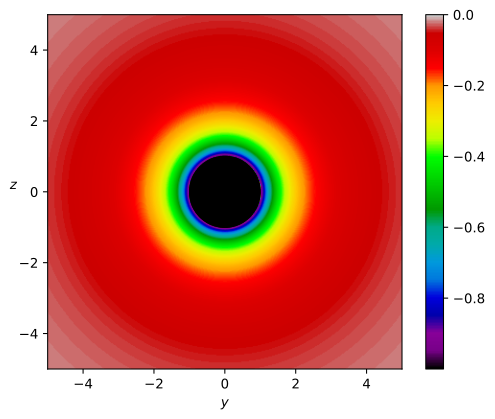
\includegraphics[width=\textwidth]{images/pdf/Directional_Derivative_of_Vector_Density_norm_of_Light_from_Rest_Source.pdf}
		\caption{Rest Source}
		\label{subfig_1: directional derivative of vector density norm}
	\end{subfigure}
	\begin{subfigure}{0.45\textwidth}
		\centering
		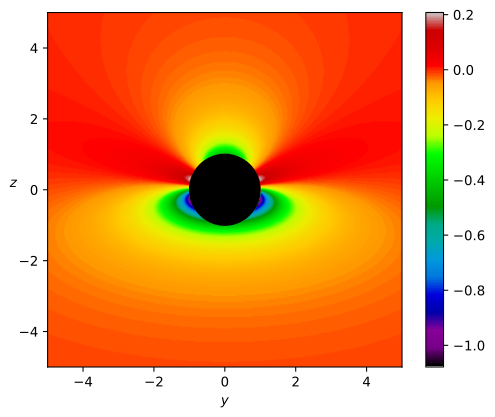
\includegraphics[width=\textwidth]{images/pdf/Directional_Derivative_of_Vector_Density_norm_of_Light_from_Moving_Source.pdf}
		\caption{Moving Source}
		\label{subfig_2: directional derivative of vector density norm}
	\end{subfigure}
	\caption{\textbf{Directional derivative of the norm of the vector density of light}. This Figure shows the rate of change of the magnitude of the vector density of light in the direction of the light's propagation $\nabla \| \underline{D} \| \cdot \hat{\underline{c}}$, at any position in the y-z plane, with the assumption $k_c\approx 0$, the values goes to infinity as we get closer to the source, so for us to be able to color the graph nicely we needed to remove the center, hence the black circle in the center.}
	\label{fig: directional derivative of vector density norm}
\end{figure}
%███████████

For the case of the moving source, we can see that it has both negative and positive values, showing the rate of change of the density in the direction of the light's propagation can change sign depending on position, which is not the case for the rest source which is consistently negative.

If you wanted to know what the directional derivative for the case of a rest source with none zero $k_c$ would be, then it would be given by the following equation which we wont derive here.

\begin{equation}
	\nabla_c \| \underline{D} \| = - \frac{2 k_\sigma^2}{r^2\sqrt{r^2 k_c^2 + k_\sigma^2}}
\end{equation}

The directional derivative has an extra term with $k_c$ in the denominator compared to the inverse square law.

\textbf{Side Note:}

Another side note is that it also happens to be that the magnitude of the gradient $\Big\| \nabla \| \underline{D} \| \Big\|$, gives the inverse square law, but it gives a different outcome for a moving source, compared to the directional derivative.
I just wanted to show the outcome of this, but I will not actually go into the math.
It is shown in the following figure.

%█████████████
\begin{figure}[H]
	\centering
	\begin{subfigure}{0.45\textwidth}
		\centering
		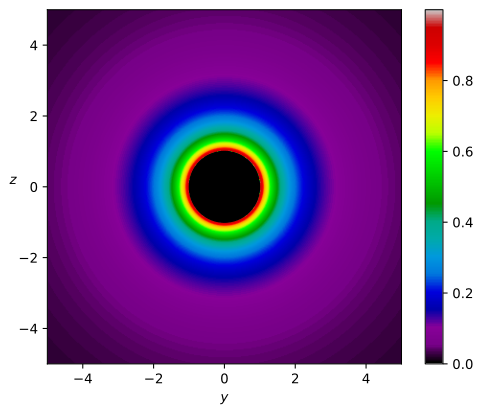
\includegraphics[width=\textwidth]{images/pdf/Density_of_Light_from_Rest_Source.pdf}
		\caption{Rest Source}
		\label{subfig_1: light emitted from a source's rate of change of vector density norm}
	\end{subfigure}
	\begin{subfigure}{0.45\textwidth}
		\centering
		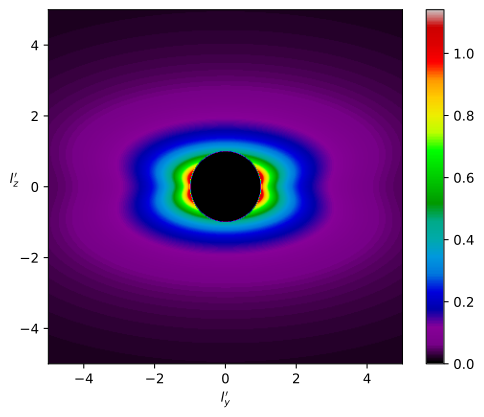
\includegraphics[width=\textwidth]{images/pdf/Rate_of_Change_of_Vector_Density_norm_of_Light_from_Moving_Source.pdf}
		\caption{Moving Source}
		\label{subfig_2: light emitted from a source's rate of change of vector density norm}
	\end{subfigure}
	\caption{\textbf{Rate of change of vector density norm of light emitted from a source}. This Figure shows the rate of change of the vector density norm of the emitted light from a source at any position in the 2d y-z plane,, with the assumption $k_c\approx 0$, the values go to infinity as we get closer to the source, so for us to be able to color the graph nicely we needed to remove the center, hence the black circle in the center.}
	\label{fig: light emitted from a source's rate of change of vector density norm}
\end{figure}
%███████████

%███████████████████████████████████████████████████████████████████
%███████████████████████████████████████████████████████████████████
\section{D'Alembert Operator on Propagation Direction}\label{sect: D'Alembert Operator on Propagation Direction}

We learnt about the D'Alembert operator in Section (\ref{sect: D'Alembert operator}):

\begin{equation}
	\square =  \frac{\partial^2}{\partial x^2} + \frac{\partial^2}{\partial y^2} + \frac{\partial^2}{\partial z^2} - \frac{1}{c^2}\frac{\partial^2}{\partial t^2}
\end{equation}

It is a Lorentz invariant quantity $\square'=\square$, so its form and how it acts on a field remain unchanged under Lorentz transformations.
It ensures that the physical predictions derived from the operator and the field it acts upon are consistent across different inertial reference frames.
It is what we will apply to the light from a source's velocity.

%, is given at $t=0$ in equation \eqref{eq: direction of light from moving source}.


If we have light being continuously emitted, evenly in all directions, from a moving point source that is currently at the origin, as shown in figure (\ref{subfig_2: full field transformation Moving Source}).
Then the light's velocity is described at each position $\underline{l}=(x,y,z)$ by the equation \eqref{eq: direction of light from moving source}.
If the source moves by $ut$ in the z-direction the displacement between the source and the position $(x,y,z)$ is now $(x,y,z-ut)$, we can substitute this into equation \eqref{eq: direction of light from moving source} to get the speed of the light at $\underline{l}$ at any time $t$.
We would then have the light's velocity described by

\begin{equation}
	\underline{\hat{c}} = \frac{1}{ \gamma \left( L - \beta \gamma (z-ut) \right) }
	\begin{pmatrix}
		x \\
		y \\
		\gamma \left(\gamma (z-ut) - \beta L \right)
	\end{pmatrix}
\end{equation}

at time $t$ with $L=\sqrt{x^2 + y^2 + (z-ut)^2}$

The reason we want to include time in the equation, is because we will need to differentiate it with respect to it.
After this we can then substitute back in $t=0$.

The derivation of $\square\underline{\hat{c}}$ gives a huge amount of terms, that take a long time to cancel down to a simple form.
So we will just show the result, which was checked with some symbolic computation software (Mathematica).

\begin{equation}
	\square \underline{\hat{c}} =
	\begin{pmatrix}
		\square \hat{c}_x \\
		\square \hat{c}_y \\
		\square \hat{c}_z
	\end{pmatrix}
	=
	- \frac{2}{L^2\gamma^2\left( 1 + \frac{u}{c} \frac{\gamma z}{L} \right)^2} \cdot \underline{\hat{c}}
\end{equation}

This is shown in the figure below.

For source at rest $u=0$, this simplifies to inverse square law $\square \underline{\hat{c}} =\frac{2}{r^2}\underline{\hat{c}}$.

%█████████████
\begin{figure}[H]
	\centering
	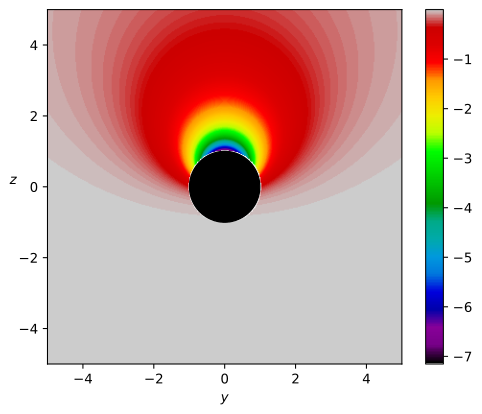
\includegraphics[width=0.9\textwidth]{images/pdf/d_alembert_operator_on_lights_velocity_unit_vector.pdf}
	\caption{\textbf{d'Alembert operator on light's velocity unit vector}. This Figure shows the d'Alembert operator applied to the unit vector of the light's velocity, it is a measure of the rate of change of the light's velocity in all directions and time, the d'Alembert operator is lorentz invariant and therefor holds the same form in all frames of reference.}
	\label{fig: d'Alembert operator on light's velocity unit vector}
\end{figure}
%███████████

%███████████████████████████████████████████████████████████████████
%███████████████████████████████████████████████████████████████████
\section{Summary}\label{sect: Summary app 2}

From this, we looked at different quantities that for a source at rest have an inverse square law $\propto 1/r^2$.

We checked for ways to get an inverse square law by using the scalar density, a vector form of the density, and for the direction of lights propagation give its position.


also using a 4 vector gradient $\nabla_4$ on the density vector magnitude $\|D\| = k_\sigma / L$

\begin{equation}
	\nabla_4 = \begin{pmatrix}
		\frac{\partial}{\partial x} \\
		\frac{\partial}{\partial y} \\
		\frac{\partial}{\partial z} \\
		\frac{1}{c} \frac{\partial}{\partial t}
	\end{pmatrix}
\end{equation}

\begin{equation}
	\left \| \nabla_4 \frac{k_\sigma }{L} \right\| = ... = \frac{k_\sigma}{L^2}
\end{equation}

need to use the time element as complex number